\documentclass[12pt,a4paper,bibliography=totocnumbered,listof=totocnumbered]{scrartcl}
\usepackage[ngerman]{babel}
\usepackage[utf8]{inputenc}
\usepackage{amsmath}
\usepackage{amsfonts}
\usepackage{amssymb}
\usepackage{graphicx}
\usepackage{fancyhdr}
\usepackage{tabularx}
\usepackage{geometry}
\usepackage{setspace}
\usepackage[right]{eurosym}
\usepackage[printonlyused]{acronym}
\usepackage{subfig}
\usepackage{floatflt}
\usepackage[usenames,dvipsnames]{color}
\usepackage{colortbl}
\usepackage{paralist}
\usepackage{array}
\usepackage{titlesec}
\usepackage{parskip}
\usepackage[right]{eurosym}
\usepackage{picins}
\usepackage[subfigure,titles]{tocloft}
\usepackage[pdfpagelabels=true]{hyperref}
\usepackage{bibgerm}

\usepackage{listings}
\lstset{basicstyle=\footnotesize, captionpos=b, breaklines=true, showstringspaces=false, tabsize=2, frame=lines, numbers=left, numberstyle=\tiny, xleftmargin=2em, framexleftmargin=2em}
\makeatletter
\def\l@lstlisting#1#2{\@dottedtocline{1}{0em}{1em}{\hspace{1,5em} Lst. #1}{#2}}
\makeatother

\geometry{a4paper, top=27mm, left=30mm, right=20mm, bottom=35mm, headsep=10mm, footskip=12mm}

\hypersetup{unicode=false, pdftoolbar=true, pdfmenubar=true, pdffitwindow=false, pdfstartview={FitH},
	pdftitle={Bericht},
	pdfauthor={Dennis Felgentreu},
	pdfsubject={Bericht},
	pdfcreator={\LaTeX\ with package \flqq hyperref\frqq},
	pdfproducer={pdfTeX \the\pdftexversion.\pdftexrevision},
	pdfkeywords={},
	pdfnewwindow=true,
	colorlinks=true,linkcolor=black,citecolor=black,filecolor=magenta,urlcolor=black}
\pdfinfo{/CreationDate (D:20141228143822)}

\begin{document}

\titlespacing{\section}{0pt}{12pt plus 4pt minus 2pt}{-6pt plus 2pt minus 2pt}

% Kopf- und Fusszeile
\renewcommand{\sectionmark}[1]{\markright{#1}}
\renewcommand{\leftmark}{\rightmark}
\pagestyle{fancy}
\lhead{}
\chead{}
\rhead{\thesection\space\contentsname}
\lfoot{Bericht zu Simulation Elektromechanischer Systeme}
\cfoot{}
\rfoot{\ Seite \thepage}
\renewcommand{\headrulewidth}{0.4pt}
\renewcommand{\footrulewidth}{0.4pt}

% Vorspann
\renewcommand{\thesection}{\Roman{section}}
\renewcommand{\theHsection}{\Roman{section}}
\pagenumbering{arabic}

% ----------------------------------------------------------------------------------------------------------
% Titelseite
% ----------------------------------------------------------------------------------------------------------
\thispagestyle{empty}
\begin{center}
	
\includegraphics[scale=0.5]{Bilder/eah-logo.png}\\
	\vspace*{2cm}
	\Large
	\textbf{Fachbereich Elektrotechnik/Informationstechnik}\\
	\textbf{Studiengang: Master Mechatrokik}\\
	\vspace*{2cm}
	\Huge
	\textbf{Bericht}\\
	\vspace*{0.5cm}
	\large
	
	Simulation Elektromechanischer Systeme\\
	
	
	\vspace*{1cm}
	\textbf{Bericht zu den Versuchen}\\
	\vspace*{2cm}
	
	\vfill
	\normalsize
	\newcolumntype{x}[1]{>{\raggedleft\arraybackslash\hspace{0pt}}p{#1}}
	\begin{tabular}{x{6cm}p{7.5cm}}
		\rule{0mm}{5ex}\textbf{Bearbeiter:} &
				 Dennis Felgentreu\newline MatrikelNr. 633374 \newline
				 Henry Pohl\newline MatrikelNr. 633374\\ 
		\rule{0mm}{5ex}\textbf{Datum:} & \today \\ 
	\end{tabular} 
\end{center}
\pagebreak

% -------------------------------------------------------------------
% Verzeichniss
% -------------------------------------------------------------------
% 

\renewcommand{\cfttabpresnum}{Tab. }
\renewcommand{\cftfigpresnum}{Abb. }
\settowidth{\cfttabnumwidth}{Abb. 10\quad}
\settowidth{\cftfignumwidth}{Abb. 10\quad}

\titlespacing{\section}{0pt}{12pt plus 4pt minus 2pt}{2pt plus 2pt minus 2pt}
\singlespacing
\rhead{INHALTSVERZEICHNIS}
\renewcommand{\contentsname}{Inhaltsverzeichnis}
\phantomsection
\addtocounter{section}{1}
\tableofcontents
\newpage

% ----------------------------------------------------------------------------------------------------------
% Formatierungen
% ----------------------------------------------------------------------------------------------------------
% Abstände Überschrift
\titlespacing{\section}{0pt}{12pt plus 4pt minus 2pt}{-6pt plus 2pt minus 2pt}
\titlespacing{\subsection}{0pt}{12pt plus 4pt minus 2pt}{-6pt plus 2pt minus 2pt}
\titlespacing{\subsubsection}{0pt}{12pt plus 4pt minus 2pt}{-6pt plus 2pt minus 2pt}

% Kopfzeile
\renewcommand{\sectionmark}[1]{\markright{#1}}
\renewcommand{\subsectionmark}[1]{}
\renewcommand{\subsubsectionmark}[1]{}
\lhead{\theHsection " " \rightmark}
\rhead{}

\onehalfspacing
\renewcommand{\thesection}{\arabic{section}}
\renewcommand{\theHsection}{\arabic{section}}
\setcounter{section}{0}

% ----------------------------------------------------------------------------------------------------------
% Tauchspule
% ----------------------------------------------------------------------------------------------------------
\section{Simulation eines Tauchspulenantriebes mit Matlab}

Bei diesem Versuch soll ein Tauchspulenantrieb Simuliert werden. Dabei wird das reale System in eine Zustandsgleichung überführt und mithilfe des Programmes Matlab simuliert. Die dabei gewonnenen Simulationsergebnisse sollen anschließend mit einem realen Versuchsaufbau verglichen werden.
Bei diesem Vergleich wird ins besondere das Frequenzverhalten untersucht.

\subsection{Vorbereitung}



\subsubsection{Aufbau und Wirkung}

\subsubsection{mathematische Beschreibung eines Tauchspulenantriebes}

\subsubsection{Systembeschreibung mittels Zustandsgleichungen}

\subsubsection{Zustandsgleichung für ein mechanisches System}

\subsection{Simulation mit eingeprägten Strom \\ und starr gekoppelter Masse}

\subsection{Simulation mit eingeprägter Spannung \\ und starr gekoppelter Masse}

\subsection{Simulation mit eingeprägter Spannung \\ und elastisch gekoppelter Masse}

\begin{figure}[h]
\centering
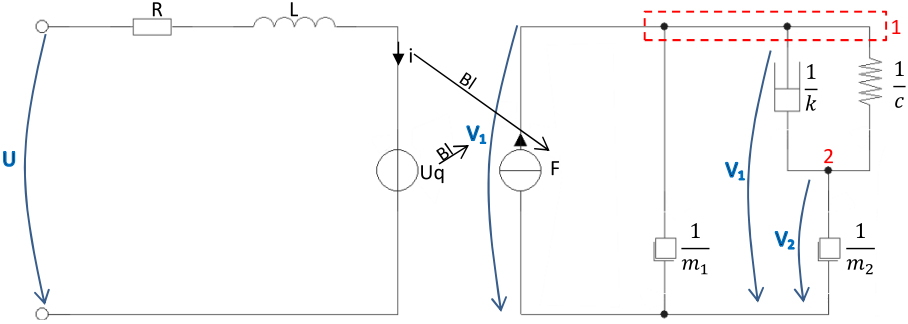
\includegraphics[width=0.7\linewidth]{Bilder/SchaltungTauchspuleAufgabe6_3.png}
\caption[]{Ersatzschaltbild Des Tauchspulenantriebes mit \\ elastisch gekoppelter Masse}
\label{fig:Schaltung6.3}
\end{figure}

\subsection{Experimentelle Überprüfung der Simulationsergebnisse}

% ----------------------------------------------------------------------------------------------------------
% Kapitel
% ----------------------------------------------------------------------------------------------------------
\pagebreak{}
\section{Netzwerksimulation eines Piezoaktor mit Simplorer}

\subsection{Vorbereitung}

\subsubsection{Netzwerkmodelle von Piezoaktoren}

\subsubsection{Ermittlung System-beschreibender Werte}

\subsection{Analytische Berechnung unter Annahme eines Einmassensystems}

\subsection{Netzwerksimulation unter Annahme eines Einmassensystems}

\subsection{Netzwerksimulation mit starr gekoppelter Zusatzmasse}

\subsection{Analytische Berechnung unter Annahme eines Zweimassensystems}

\subsection{Netzwerksimulation mit elastisch gekoppelter Last}

\subsection{Experimentelle Überprüfung der Simulationsergebnisse}


\pagebreak
% ----------------------------------------------------------------------------------------------------------
% Kapitel
% ----------------------------------------------------------------------------------------------------------
\pagebreak{}
\section{Simulation eines Positioniersystems mit Matlab/Simulink}

\subsection{Vorbereitung}

\subsubsection{Typische Positionierungsverläufe}

\subsubsection{Ermittlung System-beschreibender Werte}

\subsubsection{Wirkungsweise eines 4 Quadraten Pulsstellers}

\subsection{ --- }

\subsection{ --- }

\subsection{ --- }

\subsection{Experimentelle Überprüfung der Simulationsergebnisse}


\pagebreak

% ----------------------------------------------------------------------------------------------------------
% Literatur
% ----------------------------------------------------------------------------------------------------------
\renewcommand\refname{Quellenverzeichnis}
\bibliographystyle{geralpha}
\bibliography{bibo}
\end{document}
